\documentclass[12pt]{article}
\usepackage{amsmath,amssymb,amsthm,bm,setspace,geometry,pgfplots}
\pgfplotsset{compat=1.18}
\geometry{margin=1in}
\onehalfspacing

\begin{document}

\title{Two-Period Consumption--Saving Problem with Lognormal Income Risk}
\author{}
\date{}
\maketitle

\section{Setup}

The representative agent maximizes expected lifetime utility
\begin{equation}
    \max_{s \in [0,y_1]} \; \log(c_1) + \beta \, \mathbb{E}[\log(c_2)],
\end{equation}
where
\[
c_1 = y_1 - s, 
\qquad
c_2 = (1+\lambda) x z_2 + s,
\]
and \( z_2 \sim \log\mathcal{N}(0,\sigma^2) \), so that \( \mathbb{E}[z_2] = e^{\sigma^2/2} \).

The parameter \( \lambda \) scales the second-period endowment, \( x>0 \) is a baseline level, and \( \beta \in (0,1) \) is the discount factor.

---

\section{Exact First-Order Condition}

The first-order condition (Euler equation) for an interior optimum is
\begin{equation}
    \frac{1}{y_1 - s} 
    = 
    \beta \, \mathbb{E}\!\left[\frac{1}{s + (1+\lambda)x z_2}\right].
    \label{eq:Euler}
\end{equation}
Because the left-hand side is increasing and the right-hand side is decreasing in \(s\), the solution is unique whenever it lies in the interior \((0,y_1)\).

---

\section{Second-Order Approximation}

Define
\[
\mu \equiv \mathbb{E}[z_2] = e^{\sigma^2/2}, 
\qquad
v \equiv \operatorname{Var}\big((1+\lambda)x z_2\big) 
     = (1+\lambda)^2 x^2 e^{\sigma^2}\big(e^{\sigma^2}-1\big).
\]
Using a second-order (delta-method) approximation,
\[
\mathbb{E}[\log(s+(1+\lambda)xz_2)]
\approx 
\log\big(s+(1+\lambda)x\mu\big)
-\frac{v}{2\big(s+(1+\lambda)x\mu\big)^2}.
\]

The approximate objective is then
\begin{equation}
    \max_{0\le s \le y_1}\;
    \log(y_1 - s)
    + \beta\!\left[
        \log\big(s+(1+\lambda)x\mu\big)
        - \frac{v}{2\big(s+(1+\lambda)x\mu\big)^2}
    \right].
\end{equation}

---

\subsection*{First-Order Condition (Approximate)}

The first-order condition becomes
\begin{equation}
    \frac{1}{y_1 - s}
    = \beta\!\left[
        \frac{1}{m}
        + \frac{v}{m^3}
    \right],
    \qquad
    m \equiv s + (1+\lambda)x\mu.
\end{equation}
Let \(a = (1+\lambda)x\mu\) and \(b = y_1 + a\).  
If we set \(v=0\), we obtain the certainty-equivalent (CE) solution:
\begin{align}
m_0 &= \frac{\beta b}{1+\beta},
&
s_{\mathrm{CE}} &= \frac{\beta y_1 - a}{1+\beta}.
\end{align}

---

\subsection*{Precautionary Correction}

Linearizing FOC around \(m_0\) for small \(v\) gives
\[
\delta m = \frac{v}{(1+\beta)m_0},
\qquad
s^\star \approx s_{\mathrm{CE}} + \frac{v}{(1+\beta)m_0}.
\]
Substituting \(m_0=\tfrac{\beta(y_1+a)}{1+\beta}\) yields
\begin{equation}
\boxed{
s^\star(\lambda)
\;\approx\;
\frac{\beta y_1 - (1+\lambda)x e^{\sigma^2/2}}{1+\beta}
\;+\;
\frac{(1+\lambda)^2 x^2 e^{\sigma^2}\!\big(e^{\sigma^2}-1\big)}
{\beta\big[y_1 + (1+\lambda)x e^{\sigma^2/2}\big]}.
}
\label{eq:s_approx}
\end{equation}
The first term is the certainty-equivalent saving, and the second term is the \emph{precautionary saving correction}, which is positive and increasing in \(\sigma\).

---

\section{Comparative Statics with Respect to \(\lambda\)}

Let
\[
A \equiv x e^{\sigma^2/2},
\qquad
K \equiv e^{\sigma^2}\big(e^{\sigma^2}-1\big),
\qquad
t \equiv 1+\lambda,
\qquad
B \equiv \frac{x^2 K}{\beta}.
\]
Then equation~\eqref{eq:s_approx} can be written compactly as
\begin{equation}
s^\star(\lambda)
=
\frac{\beta y_1 - tA}{1+\beta}
+ 
B\cdot \frac{t^2}{y_1 + tA}.
\end{equation}

The derivative with respect to \(\lambda\) is
\begin{equation}
\frac{d s^\star}{d\lambda}
=
-\frac{A}{1+\beta}
+
B\cdot\frac{t(2y_1 + tA)}{(y_1 + tA)^2}.
\label{eq:dsdl}
\end{equation}
\begin{itemize}
    \item The first term is negative (higher mean future income lowers saving).
    \item The second term is positive (larger income scale increases risk and hence precautionary saving).
\end{itemize}
Thus, the total effect is \emph{ambiguous}, depending on the magnitude of risk and the discount factor.

\subsection*{Convexity in \(\lambda\)}

Differentiating again,
\begin{equation}
\frac{d^2 s^\star}{d\lambda^2}
=
B \cdot \frac{2y_1^2}{(y_1 + tA)^3} > 0,
\end{equation}
so \( s^\star(\lambda) \) is \textbf{convex} in \(\lambda\).  
This means the marginal effect of \(\lambda\) on saving becomes less negative (or more positive) as \(\lambda\) rises.

In other words, the crowd-in effect (precautionary saving) of \(\lambda\) on saving becomes stronger as \(\lambda\) rises. As the AI shock reduces \(\lambda\) for the mover from low to middle sector, the crowd-in effect is weaker and therefore a reduction of saving for the middle sector. On the other hand, the AI shock enlarges \(\lambda\) for the mover from middle to high sector, the crowd-in effect is stronger and therefore an increase of saving for the high sector.

---

\section{Comparative Statics with Respect to \(y_1\)}

From the approximate solution \eqref{eq:s_approx}, we can derive the effect of first-period income on optimal saving:
\begin{equation}
\frac{\partial s^\star}{\partial y_1}
=
\frac{\beta}{1+\beta}
-
B\cdot\frac{t^2}{(y_1 + tA)^2}.
\label{eq:dsdy1}
\end{equation}

This derivative has two components:
\begin{itemize}
    \item \textbf{Direct consumption-smoothing effect} (first term): $\frac{\beta}{1+\beta} > 0$
    \begin{itemize}
        \item Higher $y_1$ increases saving to smooth consumption across periods
        \item This is the standard life-cycle saving motive
    \end{itemize}
    \item \textbf{Precautionary adjustment} (second term): $-B\cdot\frac{t^2}{(y_1 + tA)^2} < 0$
    \begin{itemize}
        \item Higher $y_1$ reduces the relative importance of precautionary saving
        \item With more first-period resources, the agent is less concerned about second-period risk
    \end{itemize}
\end{itemize}

\subsection*{Net Effect}

The net effect $\frac{\partial s^\star}{\partial y_1}$ is \textbf{ambiguous} and depends on parameter values and the level of $y_1$: 
\begin{equation}
    \frac{\partial s^\star}{\partial y_1} > 0 \quad \Leftrightarrow \quad \frac{\beta}{1+\beta} > B\cdot\frac{t^2}{(y_1 + tA)^2}
\end{equation}

If the inequality for $\frac{\partial s^\star}{\partial y_1} > 0$ holds at $y_1=0$, it is a sufficient condition for it to hold for all $y_1\geq 0$. Plugging $y_1=0$ into the condition gives:
\begin{equation}
\frac{\beta}{1+\beta} > B \cdot \frac{1}{A^2}
\end{equation}
Recall that $A = (1+\lambda)x e^{\sigma^2/2}$ and $B = \frac{(1+\lambda)^2 x^2 e^{\sigma^2} (e^{\sigma^2}-1)}{\beta}$, so
\[
B \cdot \frac{1}{A^2} 
= 
\frac{(1+\lambda)^2 x^2 e^{\sigma^2} (e^{\sigma^2}-1)}{\beta} \cdot \frac{1}{(1+\lambda)^2 x^2 e^{\sigma^2}} 
= 
\frac{e^{\sigma^2}-1}{\beta}
\]
Thus, the sufficient condition becomes
\begin{equation}
\frac{\beta}{1+\beta} > \frac{e^{\sigma^2}-1}{\beta}
\end{equation}
or equivalently,
\begin{equation}
e^{\sigma^2} < \frac{\beta^2}{1+\beta} + 1
\end{equation}
Taking logs yields the sufficient upper bound on $\sigma$:
\begin{equation}
\sigma^2 < \log\left( \frac{\beta^2}{1+\beta} + 1 \right)
\end{equation}
Therefore, if $\sigma^2$ satisfies this bound, then $\frac{\partial s^\star}{\partial y_1} > 0$ for all $y_1 \geq 0$.

The second derivative is always positive:
\begin{equation}
\frac{\partial^2 s^\star}{\partial y_1^2}
=
B\cdot\frac{2t^2}{(y_1 + tA)^3} > 0,
\end{equation}
so $s^\star(y_1)$ is \textbf{convex} in $y_1$.

\textbf{Case Analysis:}
\begin{itemize}
    \item \textbf{High $y_1$ or low risk}: $\frac{\partial s^\star}{\partial y_1} > 0$ (consumption smoothing dominates)
    \item \textbf{Low $y_1$ or high risk}: $\frac{\partial s^\star}{\partial y_1}$ could be negative (precautionary adjustment dominates)
    \item \textbf{Asymptotic behavior}: As $y_1 \to \infty$, $\frac{\partial s^\star}{\partial y_1} \to \frac{\beta}{1+\beta} > 0$
    \item \textbf{Convexity}: The marginal effect becomes less negative (or more positive) as $y_1$ increases
\end{itemize}

\subsection*{Economic Interpretation}

The convexity of $s^\star(y_1)$ captures the interaction between consumption smoothing and precautionary motives:
\begin{itemize}
    \item At \textbf{low wealth levels}, precautionary concerns may dominate, potentially leading to \emph{dissaving} (negative marginal propensity to save) as agents prioritize current consumption when future income is risky
    \item At \textbf{high wealth levels}, standard consumption smoothing dominates, and saving increases with income
    \item The convex shape reflects \textbf{diminishing precautionary motives}: as first-period wealth increases, agents become less sensitive to second-period income risk, consistent with decreasing absolute risk aversion under logarithmic utility
\end{itemize}

---

\section{Small-Risk Approximation}

For small \(\sigma^2\), use
\[
e^{\sigma^2/2}\approx 1+\frac{\sigma^2}{2},
\qquad
e^{\sigma^2}(e^{\sigma^2}-1)\approx \sigma^2.
\]
This simplifies the solution to
\begin{equation}
s^\star(\lambda)
\approx
\frac{\beta y_1 - (1+\lambda)x(1+\frac{\sigma^2}{2})}{1+\beta}
+
\frac{(1+\lambda)^2 x^2 \sigma^2}
{\beta\,[y_1 + (1+\lambda)x(1+\frac{\sigma^2}{2})]}.
\end{equation}

---

\section{Illustration}


We consider the second-order approximate solution
\[
s^\star(\lambda)
=
\frac{\beta y_1 - (1+\lambda)x e^{\sigma^2/2}}{1+\beta}
+
\frac{(1+\lambda)^2 x^2 e^{\sigma^2}\!\big(e^{\sigma^2}-1\big)}
{\beta\,[\,y_1 + (1+\lambda)x e^{\sigma^2/2}\,]}.
\]
Parameters are chosen to produce a symmetric convex pattern
\[
s^\star(-0.2) > s^\star(0) < s^\star(0.2),
\]
with both gaps of similar magnitude.

\subsection*{Parameter Values}
\begin{table}[h!]
\centering
\begin{tabular}{lcc}
\hline
Parameter & Symbol & Value \\
\hline
First-period endowment & $y_1$ & 1.0 \\
Discount factor & $\beta$ & 0.9535 \\
Scale of risky endowment & $x$ & 1.13 \\
Lognormal standard deviation & $\sigma$ & 0.681 \\
\hline
\end{tabular}
\caption{Parameterization for balanced convexity in $s^\star(\lambda)$.}
\label{tab:param_balanced}
\end{table}

\subsection*{Results}

\begin{table}[h!]
\centering
\begin{tabular}{lccc}
\hline
 & $\lambda=-0.2$ & $\lambda=0$ & $\lambda=0.2$ \\
\hline
$s^\star(\lambda)$ & 0.28011 & 0.27650 & 0.28004 \\
Gap from $\lambda=0$ & $+0.00361$ & -- & $+0.00354$ \\
\hline
\end{tabular}
\caption{Values of $s^\star(\lambda)$ showing convex pattern.}
\label{tab:s_values}
\end{table}

\begin{figure}[h!]
    \centering
    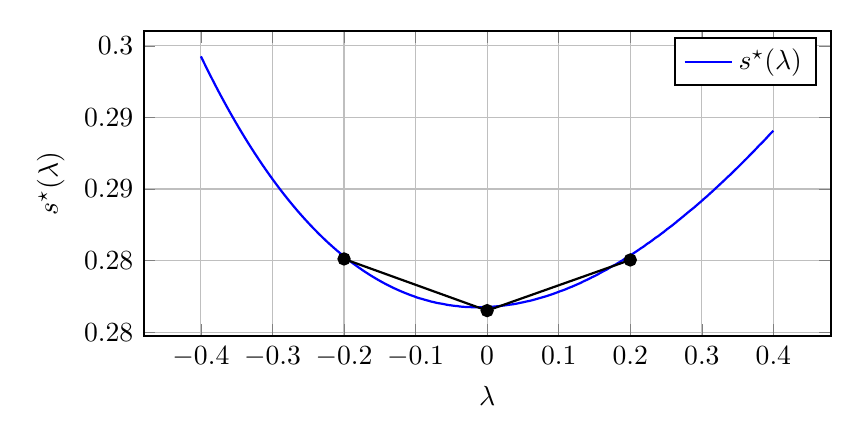
\begin{tikzpicture}
    \begin{axis}[
        width=0.85\textwidth,
        height=0.45\textwidth,
        xlabel={$\lambda$},
        ylabel={$s^\star(\lambda)$},
        grid=both,
        domain=-0.4:0.4,
        samples=200,
        thick,
    ]
    % Parameters
    \def\beta{0.9535}
    \def\yone{1.0}
    \def\x{1.13}
    \def\sigma{0.681}
    \pgfmathsetmacro{\mu}{exp(\sigma*\sigma/2)}
    \pgfmathsetmacro{\K}{exp(\sigma*\sigma)*(exp(\sigma*\sigma)-1)}
    \pgfmathsetmacro{\A}{\x*\mu}
    \pgfmathsetmacro{\B}{\x*\x*\K/\beta}
    % Plot s*(lambda)
    \addplot[blue,thick]
        ({x},{(\beta*\yone - (1+x)*\A)/(1+\beta) + \B*((1+x)^2)/(\yone + (1+x)*\A)});
    \addlegendentry{$s^\star(\lambda)$}
    % Markers
    \addplot[mark=*] coordinates {(-0.2,0.28011) (0,0.27650) (0.2,0.28004)};
    \end{axis}
    \end{tikzpicture}
    \caption{Balanced convexity of $s^\star(\lambda)$ under parameter set in Table~\ref{tab:param_balanced}.}
    \label{fig:balanced_convexity}
    \end{figure}
    
    \noindent
    The pattern confirms that $s^\star(\lambda)$ is convex: both $s^\star(-0.2)$ and $s^\star(0.2)$ exceed $s^\star(0)$, 
    illustrating symmetric precautionary adjustments to small deviations in future endowment scaling $\lambda$.

---

\section{Economic Interpretation}

\begin{itemize}
    \item For small $\lambda$, a larger future endowment reduces saving (the income effect dominates).
    \item For large $\lambda$, risk amplification dominates, raising precautionary saving.
    \item The convexity of $s^\star(\lambda)$ captures this trade-off: 
    increasing $\lambda$ both raises the mean and magnifies the uncertainty of future consumption.
\end{itemize}

\end{document}
